\chapter{Evaluation}
\label{chp:eval}

\section{Experimental Setup}

The evaluation of the tool was performed on a local machine, using the Docker-based environment described in Chapter~\ref{chp:docker}.  
The environment consisted of:

\begin{itemize}
    \item Local machine running \textbf{Ubuntu 25.04};
    %\item Docker container based on \textbf{Ubuntu 24.04};
    \item \textbf{Ghidra~11.4.2} (latest version at the time of evaluation);
    \item \textbf{Jadx~1.5.3} (latest version at the time of evaluation);
    \item \textbf{GhidraMCP~1.4} (latest version at the time of evaluation);
    \item \textbf{jadx-ai-mcp~4.0.0} (latest version at the time of evaluation).
\end{itemize}

\subsection{AWS for POIROT}

The extraction of crashes used for this evaluation is described in Chapter~\ref{chp:preliminaries}, and the corresponding execution environment is detailed in Chapter~\ref{chp:preliminaries_env}.  
All POIROT runs were executed on an AWS EC2 instance configured for large-scale fuzzing.

\subsection{LLM Used}

The evaluation was conducted using the OpenAI model GPT-5.1.  
This model represented one of the most capable \glspl{llm} available at the time of testing and offered reliable support for \gls{mcp}-based tool use.
GPT-5.1 also integrates smoothly with the Pydantic framework, allowing strict control over structured outputs.

% No fine-tuning or additional training was performed, as the goal of the evaluation was to assess how a general-purpose model behaves when equipped with structured context and targeted guidance through MCP-based evidence retrieval.


\section{Test Applications}

Table~\ref{tab:apps} lists the applications used for the evaluation, together with the exact versions of each APK.  
These apps were selected from the POIROT dataset and filtered based on the run performed. %The applications may have different versions in the POIROT dataset and this dataset. \textcolor{red}{Non so se tenere questa ultima frase per sengalare che le apks hanno versioni diverse}

\begin{table}[ht]
\centering
\resizebox{1\textwidth}{!}{
\begin{tabular}{|l|l||l|l|}
\hline
\multicolumn{4}{|c|}{\textbf{Applications Used for Evaluation}} \\
\hline
\textbf{App} & \textbf{Version} & \textbf{App} & \textbf{Version} \\
\hline
br.com.pedidos10 & 1.16.4 & ca.radioplayer.android & 6.3.420.1 \\
com.ahnlab.v3mobileplus & 2.5.20.10 & com.appgeneration.itunerfree & 9.3.13 \\
com.cisco.webex.meetings & 45.3.0 & com.clearchannel.iheartradio.controller & 10.36.0 \\
com.ford.fordpasseu & 4.23.1 & com.hyundaicard.cultureapp & 1.0.72 \\
com.intsig.BCRLite & 7.85.5 & com.jeju.genie & 2.2.13 \\
com.kbstar.kbbridge & 1.2.1 & com.kt.ktauth & 02.01.37 \\
com.lottemembers.android & 7.7.5 & com.more.dayzsurvival.gp & 25.1002.1 \\
com.pandora.android & 2509.1 & com.rockbite.deeptown & 6.2.10 \\
com.rstgames.durak & 1.9.11 & com.samsungcard.shopping & 1.4.901 \\
com.skmc.okcashbag.home\_google & 7.0.8 & com.skt.prod.dialer & 13.6.5 \\
com.skt.smartbill & 6.4.1 & com.sopheos.videgreniersmobile & 20.11.10 \\
com.ssg.serviceapp.android.egiftcertificate & 2.6.10 & com.teamjin.deliveryk & 7.0.3 \\
com.tencent.mm & 8.0.28 & com.tplink.skylight & 3.1.20 \\
fr.radioplayer.android & 6.6.420.1 & kr.co.busanbank.mbp & 3.0.10 \\
kr.co.morpheus.geps & 02.42 & kr.co.samsungcard.mpocket & 5.4.306 \\
kr.go.iros & 1.2.3 & kr.go.kcs.mobile.pubservice & 1.0.281 \\
kr.go.minwon.m & 2.5.95 & kr.go.nts.android & 12.8 \\
kr.go.wetax.android & 5.4.14 & nh.smart.allonebank & 1.8.8 \\
nh.smart.banking & 4.1.2 & nh.smart.card & 6.5.0 \\
nh.smart.nhcok & 2.0.70 & ragazzo.alphacode.com.br & 3.0.9 \\
tw.com.taishinbank.ccapp & 5.631 & tw.gov.tra.twtraffic & 2.1.2 \\
\hline
\end{tabular}
}
\caption{Applications evaluated by the triage system.}
\label{tab:apps}
\end{table}

\textcolor{red}{Devo scrivere quali sono lastversion e quali quelle di circa 2023? }

Across all these applications, a total of 59 methods were identified, each associated with one or more crashes.  
In total, the dataset contained 134 crash instances.

\subsection{Execution Time}

Table~\ref{tab:apps_time} reports the execution time for each application.  
The total time per APK depends primarily on the \emph{number of crashes} produced by POIROT, as well as the number of relevant libraries and the complexity of the stack trace.
Note that the reported time covers only the \gls{llm} classification phase and does not include the startup time of Ghidra, which depends solely on the number and size of the native libraries being imported.

\begin{table}[ht]
\centering
\resizebox{1\textwidth}{!}{
\begin{tabular}{|l|l||l|l|}
\hline
\multicolumn{4}{|c|}{\textbf{Execution LLM Time per Application}} \\
\hline
\textbf{App} & \textbf{Time (s)} & \textbf{App} & \textbf{Time (s)} \\
\hline
br.com.pedidos10 & 80 & ca.radioplayer.android & 480 \\ 
com.ahnlab.v3mobileplus & 338 & com.appgeneration.itunerfree & 113 \\ 
com.cisco.webex.meetings & 129 & com.clearchannel.iheartradio.controller & 200 \\ 
com.ford.fordpasseu & 185 & com.hyundaicard.cultureapp & 48 \\ 
com.intsig.BCRLite & 59 & com.jeju.genie & 33 \\ 
com.kbstar.kbbridge & 35 & com.kt.ktauth & 28 \\ 
com.lottemembers.android & 71 & com.more.dayzsurvival.gp & 25 \\ 
com.pandora.android & 420 & com.rockbite.deeptown & 17 \\ 
com.rstgames.durak & 36 & com.samsungcard.shopping & 22 \\ 
com.skmc.okcashbag.home\_google & 57 & com.skt.prod.dialer & 278 \\ 
com.skt.smartbill & 579 & com.sopheos.videgreniersmobile & 60 \\ 
com.ssg.serviceapp.android.egiftcertificate & 31 & com.teamjin.deliveryk & 83 \\ 
com.tencent.mm & 321 & com.tplink.skylight & 71 \\ 
fr.radioplayer.android & 628 & kr.co.busanbank.mbp & 805 \\ 
kr.co.morpheus.geps & 59 & kr.co.samsungcard.mpocket & 55 \\ 
kr.go.iros & 43 & kr.go.kcs.mobile.pubservice & 60 \\ 
kr.go.minwon.m & 30 & kr.go.nts.android & 87 \\ 
kr.go.wetax.android & 35 & nh.smart.allonebank & 36 \\ 
nh.smart.banking & 29 & nh.smart.card & 30 \\ 
nh.smart.nhcok & 37 & ragazzo.alphacode.com.br & 87 \\ 
tw.com.taishinbank.ccapp & 98 & tw.gov.tra.twtraffic & 78 \\ 

\hline
\hline
\multicolumn{2}{|r||}{\textbf{Average Time}} & \multicolumn{2}{l|}{\textbf{142}} \\
\hline
\end{tabular}
}
\caption{Approximate execution time per application.}
\label{tab:apps_time}
\end{table}

\subsection{Tokens usage}

\glspl{llm}, when accessed through their cloud \glspl{api}, compute usage costs based on the number of \emph{input tokens} (the prompt sent to the model) and \emph{output tokens} (the generated response).  
Token consumption plays a central role in both performance and cost.  
In this evaluation, usage varies primarily according to the size of the prompts (which include both the system and user components), the number of crashes produced by POIROT for each application, the amount of decompiled code retrieved from Ghidra—which grows with the depth and complexity of the stack trace—and the verbosity of the final triage explanation generated by the \gls{llm}.  


Table~\ref{tab:apps_tokens} reports input and output token usage for each application.

\begin{table}[ht]
\centering
\resizebox{1\textwidth}{!}{
\begin{tabular}{|l|l|l||l|l|l|}
\hline
\multicolumn{6}{|c|}{\textbf{Token Usage per Application}} \\
\hline
\textbf{App} & \textbf{Input} & \textbf{Output} &
\textbf{App} & \textbf{Input} & \textbf{Output} \\
\hline
br.com.pedidos10 & 36344 & 4006 & ca.radioplayer.android & 494465 & 23484 \\ 
com.ahnlab.v3mobileplus & 392719 & 17831 & com.appgeneration.itunerfree & 53776 & 6516 \\ 
com.cisco.webex.meetings & 92548 & 7643 & com.clearchannel.iheartradio.controller & 151439 & 7039 \\ 
com.ford.fordpasseu & 84360 & 6811 & com.hyundaicard.cultureapp & 14153 & 2152 \\ 
com.intsig.BCRLite & 33230 & 4095 & com.jeju.genie & 12987 & 2244 \\ 
com.kbstar.kbbridge & 13014 & 2189 & com.kt.ktauth & 41470 & 1466 \\ 
com.lottemembers.android & 38747 & 2655 & com.more.dayzsurvival.gp & 6542 & 1250 \\ 
com.pandora.android & 70891 & 9638 & com.rockbite.deeptown & 6564 & 1421 \\ 
com.rstgames.durak & 19232 & 1726 & com.samsungcard.shopping & 12380 & 1170 \\ 
com.skmc.okcashbag.home\_google & 30012 & 3708 & com.skt.prod.dialer & 212223 & 12100 \\ 
com.skt.smartbill & 359973 & 28820 & com.sopheos.videgreniersmobile & 48392 & 3213 \\ 
com.ssg.serviceapp.android.egiftcertificate & 18401 & 1734 & com.teamjin.deliveryk & 31816 & 4143 \\ 
com.tencent.mm & 877501 & 16197 & com.tplink.skylight & 29527 & 4077 \\ 
fr.radioplayer.android & 202292 & 21668 & kr.co.busanbank.mbp & 495055 & 44584 \\ 
kr.co.morpheus.geps & 22248 & 1544 & kr.co.samsungcard.mpocket & 29228 & 2915 \\ 
kr.go.iros & 24988 & 2374 & kr.go.kcs.mobile.pubservice & 25362 & 3232 \\ 
kr.go.minwon.m & 14516 & 1378 & kr.go.nts.android & 59025 & 4887 \\ 
kr.go.wetax.android & 12829 & 2305 & nh.smart.allonebank & 24960 & 1695 \\ 
nh.smart.banking & 20250 & 1610 & nh.smart.card & 14111 & 1783 \\ 
nh.smart.nhcok & 14361 & 1676 & ragazzo.alphacode.com.br & 38671 & 3792 \\ 
tw.com.taishinbank.ccapp & 31781 & 4205 & tw.gov.tra.twtraffic & 42834 & 3530 \\ 

\hline
\hline
\multicolumn{3}{|r||}{\textbf{Average Input Tokens}} &
\multicolumn{3}{l|}{\textbf{212434}} \\
\multicolumn{3}{|r||}{\textbf{Average Output Tokens}} &
\multicolumn{3}{l|}{\textbf{13963}} \\
\hline
\end{tabular}
}
\caption{Input and output token usage per application.}
\label{tab:apps_tokens}
\end{table}

\subsection{Requests and Tool Calls}

Each crash triggers a series of \emph{LLM requests}, corresponding to the number of times the agent sends a prompt to the model, and a number of \emph{LLM tool calls}, which represent successful invocations of Jadx or Ghidra through MCP during the analysis.  

Table~\ref{tab:apps_requests} reports, for each application, the number of LLM requests and MCP tool calls performed during the full triage stage.  

\begin{table}[ht]
\centering
\resizebox{1\textwidth}{!}{
\begin{tabular}{|l|l|l||l|l|l|}
\hline
\multicolumn{6}{|c|}{\textbf{LLM request and Tool Calls per Application}} \\
\hline
\textbf{App} & \textbf{Input} & \textbf{Output} &
\textbf{App} & \textbf{Input} & \textbf{Output} \\
\hline
br.com.pedidos10 & 5 & 9 & ca.radioplayer.android & 44 & 53 \\ 
com.ahnlab.v3mobileplus & 31 & 42 & com.appgeneration.itunerfree & 6 & 14 \\ 
com.cisco.webex.meetings & 10 & 23 & com.clearchannel.iheartradio.controller & 17 & 20 \\ 
com.ford.fordpasseu & 9 & 26 & com.hyundaicard.cultureapp & 2 & 3 \\ 
com.intsig.BCRLite & 4 & 9 & com.jeju.genie & 2 & 3 \\ 
com.kbstar.kbbridge & 2 & 3 & com.kt.ktauth & 6 & 6 \\ 
com.lottemembers.android & 2 & 5 & com.more.dayzsurvival.gp & 2 & 3 \\ 
com.pandora.android & 8 & 20 & com.rockbite.deeptown & 2 & 2 \\ 
com.rstgames.durak & 3 & 3 & com.samsungcard.shopping & 2 & 2 \\ 
com.skmc.okcashbag.home\_google & 4 & 5 & com.skt.prod.dialer & 26 & 26 \\ 
com.skt.smartbill & 51 & 82 & com.sopheos.videgreniersmobile & 6 & 10 \\ 
com.ssg.serviceapp.android.egiftcertificate & 3 & 2 & com.teamjin.deliveryk & 4 & 9 \\ 
com.tencent.mm & 49 & 42 & com.tplink.skylight & 4 & 9 \\ 
fr.radioplayer.android & 22 & 59 & kr.co.busanbank.mbp & 55 & 63 \\ 
kr.co.morpheus.geps & 3 & 4 & kr.co.samsungcard.mpocket & 4 & 8 \\ 
kr.go.iros & 4 & 4 & kr.go.kcs.mobile.pubservice & 4 & 4 \\ 
kr.go.minwon.m & 2 & 4 & kr.go.nts.android & 8 & 13 \\ 
kr.go.wetax.android & 2 & 3 & nh.smart.allonebank & 4 & 4 \\ 
nh.smart.banking & 3 & 4 & nh.smart.card & 2 & 3 \\ 
nh.smart.nhcok & 2 & 4 & ragazzo.alphacode.com.br & 5 & 13 \\ 
tw.com.taishinbank.ccapp & 4 & 10 & tw.gov.tra.twtraffic & 5 & 13 \\ 

\hline
\hline
\multicolumn{3}{|r||}{\textbf{Average LLM requests}} &
\multicolumn{3}{l|}{\textbf{16.4}} \\
\multicolumn{3}{|r||}{\textbf{Average LLM Tool Calls}} &
\multicolumn{3}{l|}{\textbf{25.3}} \\
\hline
\end{tabular}
}
\caption{LLM request and Tool Calls per application.}
\label{tab:apps_requests}
\end{table}
        
\vfill


\section{Evaluation Metrics}
\textcolor{red}{non se serve specificare le metriche}


To objectively assess the performance of the LLM-based triage system, standard information retrieval metrics derived from a confusion matrix are employed. Given the binary nature of the classification task—determining whether a crash is a vulnerability or a benign issue—the possible outcomes are defined as follows:

\begin{itemize}
    \item \textbf{True Positive (TP):} A vulnerability correctly identified by the model. The crash represents a security risk, and the system correctly classified it as such (\texttt{is\_vulnerable: true}).
    \item \textbf{False Positive (FP):} A benign crash incorrectly flagged as a vulnerability. This represents a ''false alarm``, where the model assigns security relevance to a non-exploitable issue.
    \item \textbf{True Negative (TN):} A benign crash correctly identified as non-vulnerable. The system correctly determined that the issue does not pose a security risk.
    \item \textbf{False Negative (FN):} A vulnerability missed by the model. The crash is dangerous, but the system incorrectly classified it as benign.
\end{itemize}

Based on these definitions, the following metrics were calculated:

\paragraph{Accuracy}
Accuracy measures the overall correctness of the model across all predictions. While useful, it can be misleading in datasets with significant class imbalance (e.g., where benign crashes vastly outnumber vulnerabilities).
\[
\text{Accuracy} = \frac{\text{TP} + \text{TN}}{\text{TP} + \text{TN} + \text{FP} + \text{FN}}
\]

\paragraph{Precision} Precision quantifies the reliability of the positive predictions. In the context of this thesis, high precision implies that when the tool flags a crash as a vulnerability, it is highly likely to be a genuine threat, thereby reducing the manual verification effort for analysts.
\[
\text{Precision} = \frac{\text{TP}}{\text{TP} + \text{FP}}
\]

\paragraph{Recall}
Recall measures the system's ability to detect all actual vulnerabilities. High recall is critical in security contexts to ensure that dangerous flaws are not overlooked (minimizing False Negatives).
\[
\text{Recall} = \frac{\text{TP}}{\text{TP} + \text{FN}}
\]

\paragraph{F1-Score}
For the evaluation, the F1-score was selected as the primary metric. This measure is commonly employed in classification settings because it offers a single value that reflects the trade-off between precision and recall, which is especially important when the distribution of classes is unbalanced or when both false positives and false negatives carry comparable weight. The F1-score is defined as the harmonic mean of precision and recall:
\[
\mathrm{F1} = 2 \cdot \frac{\text{precision} \cdot \text{recall}}{\text{precision} + \text{recall}}
\]
The F1-score ensures a lower overall score if either precision or recall diverges significantly, even if one of the two is high, providing a balanced view of the model's effectiveness.

\section{Results}

\begin{figure}[ht]
\centering
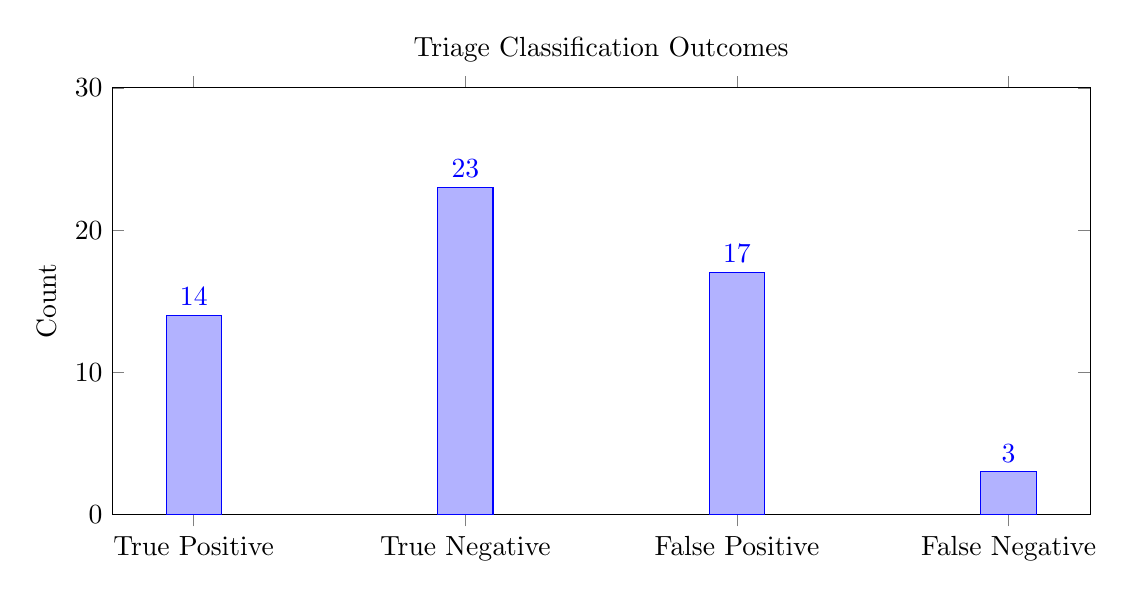
\begin{tikzpicture}
\begin{axis}[
    ybar,
    ymin=0,
    ymax=30,
    bar width=20pt,
    width=14cm,
    height=7cm,
    ylabel={Count},
    symbolic x coords={TP,TN,FP,FN},
    xticklabels={
        {True~Positive},
        {True~Negative},
        {False~Positive},
        {False~Negative}
    },
    xtick=data,
    nodes near coords,
    nodes near coords align={vertical},
    title={Triage Classification Outcomes},
]
\addplot coordinates {(TP,14) (TN,23) (FP,17) (FN,3)};
\end{axis}
\end{tikzpicture}
\caption{Distribution of classification outcomes across the dataset.}
\label{fig:classification_outcomes}
\end{figure}


The bar chart in Figure~\ref{fig:classification_outcomes} summarises how the system classified the 134 crash instances in the dataset.  
Most predictions fall into the True Negative (23) and False Positive (17) categories, indicating that the model frequently flagged benign crashes as vulnerabilities.  
Conversely, the system correctly identified 14 genuine vulnerabilities (True Positives) and missed only 3 (False Negatives).  
This distribution suggests that the model favours recall—successfully detecting most real vulnerabilities—but at the cost of a higher number of false alarms.

\begin{table}[ht]
\centering
\begin{tabular}{|l|c|}
\hline
\textbf{Metric} & \textbf{Value} \\
\hline
\hline
Accuracy  & 0.6491 \\
Precision & 0.4516 \\
Recall    & 0.8235 \\
F1 Score  & 0.2917 \\
\hline
\end{tabular}
\caption{Evaluation metrics computed from the classification results.}
\label{tab:eval_metrics}
\end{table}



Table~\ref{tab:eval_metrics} reports the derived performance metrics.  
The overall accuracy (0.6491) reflects the proportion of correct classifications across all crashes, though it is influenced by the imbalance between benign and vulnerable samples.  
Precision (0.4516) is relatively low, consistent with the high number of False Positives observed in the chart; many issues flagged as vulnerabilities did not correspond to real security risks.  
Recall (0.8235) is considerably higher, showing that the system is effective at capturing genuine vulnerabilities and rarely overlooks dangerous cases.  
However, the F1-score (0.2917)—the harmonic mean of precision and recall—is low, indicating an uneven balance between detecting vulnerabilities and avoiding false alarms.

Overall, these results show that the current implementation is conservative in its judgement, prioritising the detection of potential vulnerabilities over strict precision.  
While this behaviour is desirable in contexts where missing a vulnerability is more costly than over-reporting, it also highlights the need for improvements aimed at reducing false positives, such as integrating specialised models, adopting RAG-based grounding, or leveraging persistent agents as discussed in Chapter~\ref{chp:futureWork}.
